% Q7 Track O / Task F5 — arXiv preprint. Build: make (tectonic).
\documentclass[10pt,twocolumn]{article}
\usepackage[margin=0.75in]{geometry}
\usepackage{amsmath,amssymb}
\usepackage{graphicx}
\usepackage{booktabs}
\usepackage{array}
\usepackage{siunitx}
\usepackage{xcolor}
\usepackage[hidelinks]{hyperref}
\usepackage{microtype}
\usepackage[numbers,sort&compress]{natbib}
\graphicspath{{figs/}}
\sisetup{range-phrase=--,range-units=single}
\newcommand{\alephsim}{\textsf{aleph}}
\newcommand{\gross}{$[[144,12,12]]$}

\title{A sub-microsecond relay-BP decoder for the $[[144,12,12]]$ gross code:\\
from a fixed-point golden model to FPGA silicon and a 7\,nm predictive ASIC}
\author{Ruslan Malymon}
\date{\today}

\begin{document}
\maketitle

\begin{abstract}
We report a complete hardware implementation path for real-time decoding of the \gross{} gross
bivariate-bicycle code with relay belief propagation (relay-BP): a fixed-point golden model,
a family of banked FPGA cores, silicon campaigns, and a placed-and-routed design on a 7\,nm
predictive PDK. An 8-bit (Q5.3) min-sum message word reproduces the floating-point logical error
rate within statistical error, and a $6\times10$ leg/iteration schedule is chosen from a budget
sweep. The shipped Kria KV260 build (16/48 banking) decodes a circuit-level detector-error-model
window in \SI{15.64}{\micro\second} worst case and \SI{0.85}{\micro\second} median with early exit
at \SI{133.3}{\mega\hertz}, and is bit-exact against the software golden over $10^6$ shots at each of
three operating points. The decoder's convergence flag heralds nearly every logical error:
$P(\text{error}\mid\text{converged}) \le 3\times10^{-6}$, so the logical error rate is, to within
statistics, the non-convergence rate, and every post-processing fallback we tried was worse than
flagging alone. The full-parallel 144/864 geometry decodes in 543 cycles; it places and routes at
\SI{76.3}{\percent} of a Virtex UltraScale+ VU47P at \SI{97.3}{\mega\hertz} (\SI{5.58}{\micro\second})
and, through OpenROAD on ASAP7, at \SI{614.6}{\mega\hertz} (\SI{0.88}{\micro\second}). Gate-level
simulation of the routed 16/48 netlist gives a real-activity power of \SI{0.149}{\watt} at \SI{1}{\giga\hertz},
\SI{0.31}{\micro\joule} per decode window, \SI{93}{\percent} of it in the clock tree and register
clocking. The same simulation exposes an unrepaired hold failure on the latch register file that
makes every setup-only frequency figure provisional; we report it rather than hide it. All RTL,
goldens, campaign data and a one-command KV260 deployment are open source.

\end{abstract}

\section{Introduction}

Quantum low-density parity-check (qLDPC) codes promise fault-tolerant memory at a fraction of the
surface code's qubit overhead \citep{bravyi2024gross}, and belief-propagation decoders --- in
particular relay-BP \citep{muller2025relaybp} --- have been shown, in software, to reach the logical
error rates that make such codes useful without an ordered-statistics tail. Whether that translates
into a decoder that keeps up with a quantum processor is a hardware question: the decode of one
syndrome window must complete in about a microsecond for superconducting platforms, and in the
tens to hundreds of microseconds for ions and neutral atoms, on a budget of area and power that a
control system can absorb.

This paper documents one end-to-end answer, built in the open and measured at every step. The
contributions, in the order the work was done:

\begin{enumerate}
  \item A fixed-point relay-BP golden model for the \gross{} gross code that is the RTL specification:
        an 8-bit Q5.3 message word and a $6\times10$ schedule, each chosen by a sweep against the
        floating-point decoder on circuit-level noise (\S\ref{sec:decoder}).
  \item A ladder of synthesizable cores from a sequential FSM to a $K$-banked, constant-geometry
        design whose gather/scatter is a fixed permutation network and whose message storage is a
        latch register file, with a co-simulation harness that drives every variant --- and the
        routed ASIC netlist --- with the same golden vectors (\S\ref{sec:architecture}).
  \item Silicon results on a \$300 Kria KV260: \SI{15.64}{\micro\second} worst-case,
        \SI{0.85}{\micro\second} median, bit-exact over $3\times10^6$ shots, and the finding that the
        convergence flag heralds essentially every logical error (\S\ref{sec:silicon}).
  \item The full-parallel geometry on a rented Virtex UltraScale+ and on ASAP7 through OpenROAD:
        543 cycles, \SI{0.88}{\micro\second} at 7\,nm predictive, with the first power figure derived
        from gate-level switching activity rather than default toggle rates (\S\ref{sec:scaling}).
  \item The negative results that shaped the design and that a tape-out would have to face: no OSD
        tail, no feasible \texttt{NGROUP} setting, a streaming core that does not fit, and a
        latch-clock hold failure that repair cannot buffer away (\S\ref{sec:limitations}).
\end{enumerate}

Every number in this paper is copied from a dated report in the public repository
\citep{alephrepo}; Appendix~\ref{app:prov} maps each to its source file. Nothing measured on ASAP7
is called ``the chip'': it is a 7\,nm \emph{predictive} kit, and the target node is not.

% 02-decoder — to be written

% 03-architecture — Hardware architecture ladder (M2 → M8), gather fabrics (M9c), register file (Q7-08).
% Every figure carries a "% src:" comment naming the docs/ file and heading it was taken from.
\section{Hardware architecture}
\label{sec:architecture}

The decoder RTL was reached by a ladder of six synthesised variants, each
bit-exact against the same fixed-point golden model
(\S\ref{sec:decoder}) and each measured out-of-context (OOC) on the
target part before the next step was chosen. Table~\ref{tab:ladder}
summarises the ladder; the rest of this section explains what each step
learned. Two graph sizes appear: M2--M5 decode the code-capacity Tanner
graph of \gross{} (72~checks, 144~variables, 432~edges),
% src: docs/perf/qec-q7-fixed-bp.md M3 "Critical path — the cursor mux, not the multiply"
while M6 onward decode the circuit-level detector-error-model graph
($C=144$ checks, $N=864$ variables, $E=2952$ edges, maximum check degree~25).
% src: docs/perf/qec-q7-fixed-bp.md M6

\begin{table*}[t]
\centering
\footnotesize
\caption{Architecture ladder. Cycles are the full-schedule (no early exit)
worst case; fabric is the post-synthesis LUT count and share of the Xilinx
Kria KV260 (XCK26, 117\,120 LUTs). Clocks are OOC for M2--M5 and M9c,
the timing-met board clock for M6--M8.}
\label{tab:ladder}
\begin{tabular}{@{}llrrll@{}}
\toprule
Variant & Graph & Cycles & Fabric (LUT) & Clock / latency & Verdict \\
\midrule
M2 sequential FSM & code cap. & 28\,944 & 24\,119 (21\,\%) & 67.8\,MHz / 427\,\si{\micro\second} & cursor mux is the wall \\
% src: docs/perf/qec-q7-fixed-bp.md M2 "Honest latency headline"; M3 "Result"
M4 spatial unroll & code cap. & 301 & 94\,194 (80\,\%) & 95.2\,MHz / 3.16\,\si{\micro\second} & mux gone; arithmetic depth \\
% src: docs/perf/qec-q7-fixed-bp.md M4 "Result — the idx-mux wall is gone"
M5 SAT-overlap (6$\times$10) & code cap. & 122 & 93\,487 (79.8\,\%) & 95.9\,MHz / 1.272\,\si{\micro\second} & 1.48$\times$ free; route-bound \\
% src: docs/perf/qec-q7-fixed-bp.md M5-followup "Result — 6×10 schedule, KV260 OOC P&R"
M6 edge-serial BRAM & circuit & 672\,000 & 8\,509 (7.3\,\%) & 100\,MHz / 6.72\,ms & unroll fails to synthesise \\
% src: docs/perf/qec-q7-fixed-bp.md M6
M7 banked 12/36 & circuit & 2\,460 & 88.0\,k (75\,\%) & 75\,MHz / 32.8\,\si{\micro\second} & on silicon, 40/40 \\
% src: docs/perf/qec-q7-fixed-bp.md M7 "OOC probe sweep"; "Board + silicon"
M8 banked 16/48 & circuit & 2\,085 & 102.8\,k (88\,\%) & 133.332\,MHz / 15.64\,\si{\micro\second} & on silicon, 40/40 \\
% src: docs/perf/qec-q7-fixed-bp.md M8 "OOC probes"; "Board ladder + silicon"
M9c full-parallel gather & circuit, streaming & 4\,475 & 189\,740 (162\,\%) & 177.7\,MHz OOC & no fit on one KV260 \\
% src: docs/perf/qec-q7-fixed-bp.md M9c "Step 5 — AS-Waksman"; "area campaign — terminal verdict"
\bottomrule
\end{tabular}
\end{table*}

\subsection*{M2: sequential FSM}
The first synthesisable decoder time-multiplexes the relay-BP update into
a clocked FSM that touches one check ($\le 6$ edges) or one variable
($\le 3$ edges) per cycle, so combinational depth is bounded and independent
of graph size. One iteration is a 72-cycle check pass, a 144-cycle
variable pass (the only multiply: the memory blend
$(1-\gamma)\cdot\mathrm{computed}+\gamma\cdot m_{\mathrm{old}}$) and a
72-cycle satisfaction pass; the $4\times 25$ schedule plus a 144-cycle emit
gives a worst case of 28\,944 cycles per decode.
% src: docs/perf/qec-q7-fixed-bp.md M2 "What"; "Honest latency headline"

\subsection*{M3: out-of-context synthesis verdict}
The FSM fits both parts with no DSP and no BRAM, but at 28.3\,MHz on the
Zybo (1023\,\si{\micro\second}) and 67.8\,MHz on the KV260
(427\,\si{\micro\second}) it is two to three orders of magnitude off
real time.
% src: docs/perf/qec-q7-fixed-bp.md M3 "Result"
The binding path is not the multiply---the per-variable
$\gamma$ constants fold into LUTs and DSP usage is zero---but the runtime
check cursor: reading \texttt{BP\_CHECK\_OFF[idx]} then the edge list
synthesises to a 72-way select in front of the min-sum whose result fans
out through a 432-way write decode (net fan-outs of 586 and 626; 44 logic
levels and 74\,\% routing delay on the Zybo).
% src: docs/perf/qec-q7-fixed-bp.md M3 "Critical path — the cursor mux, not the multiply"
The lesson that shaped everything after it: on a constant-degree graph,
a runtime index into a message array is a mux tree the size of the array.

\subsection*{M4: spatial unroll}
Wiring each check's six edges and each variable's three edges as
compile-time constants deletes the cursor entirely and lets a whole BP layer
evaluate in one cycle: 301 cycles at $4\times 25$, 96$\times$ fewer than M2.
On the KV260 the unrolled datapath needs 94\,194 LUTs (80\,\%) and closes
at 95.2\,MHz, 3.16\,\si{\micro\second}---135$\times$ faster than M3; on the
Zybo it is 172.6\,\% of the part and does not fit.
% src: docs/perf/qec-q7-fixed-bp.md M4 "Result — the idx-mux wall is gone"
The new critical path is real arithmetic (the variable-update blend, 25
logic levels through five CARRY8 chains) plus routing congestion at 80\,\%
utilisation.
% src: docs/perf/qec-q7-fixed-bp.md M4 "Result"
A synthesis caveat is worth recording: with every index constant, Vivado
constant-propagated the 100-iteration message recurrence to a bogus fixed
point and deleted the datapath, leaving a 158-flop shell that ``closed
timing'' at $\sim$485\,MHz; the registers had to be anchored with
\texttt{dont\_touch}, and post-synthesis flop counts are now checked against
elaboration on every variant.
% src: docs/perf/qec-q7-fixed-bp.md M4 "Two synthesis gotchas the unroll exposed"

\subsection*{M5: the two microarchitectural levers, measured}
Adopting the LER-optimal $6\times 10$ schedule (\S\ref{sec:decoder}) cut
the cycle count to 181 and latency to 1.89\,\si{\micro\second} at
96.0\,MHz.
% src: docs/perf/qec-q7-fixed-bp.md M5 step 2 "Result — 1.68× faster than M4"
Two further levers were then tried on the KV260. \emph{SAT-overlap}
folds the syndrome check into the following check pass, since the two read
disjoint registers: 2 cycles per iteration instead of 3, 122 cycles,
1.272\,\si{\micro\second} at 95.9\,MHz on 93\,487 LUTs---a 1.48$\times$
win at unchanged clock and area.
% src: docs/perf/qec-q7-fixed-bp.md M5-followup "SAT-overlap (bp_relay_fast) — the win"
\emph{Pipelining the min-sum} is the measured negative result: splitting
the check pass raised the clock only 96.0$\to$111.3\,MHz (1.16$\times$)
against a 1.33$\times$ cycle penalty, for 2.165\,\si{\micro\second}, a 15\,\%
regression, while pushing utilisation to 85.5\,\% and worsening congestion.
% src: docs/perf/qec-q7-fixed-bp.md M5-followup "Min-sum pipeline (bp_relay_pipe) — the measured negative result"
The wall at this point is routing at $\sim$80\,\% utilisation, not logic
depth; removing work helps, adding registers does not.
% src: docs/perf/qec-q7-fixed-bp.md M5-followup "Verdict"

\subsection*{M6: the circuit-level graph does not unroll}
On the circuit-level graph (degree up to 25) neither the full unroll nor a
CHK12/VAR24 partial unroll synthesises on the KV260: Vivado's
cross-boundary area optimisation ran out of memory at $\sim$43\,GB or stalled
without progress. Only BRAM-resident edge-serial cores fit (5.5--7.3\,\%
LUT), and the two-edges-per-cycle variant gives 672\,000 cycles,
6.72\,ms at 100\,MHz on silicon.
% src: docs/perf/qec-q7-fixed-bp.md M6

\subsection*{M7: $K$-banked relay-BP}
The design space was a trilemma, all corners measured: the full spatial
unroll (144 check + 864 variable submodules) is 453\,k LUTs, 386\,\% of the
KV260; a partial unroll with a runtime group gather from flop arrays stalls
area optimisation on $O(E)$ operand muxes---the M3 cursor-mux wall again;
the banked LUTRAM store synthesises at 88\,k LUTs (75\,\%).
% src: docs/perf/qec-q7-fixed-bp.md M7 "The design space is a trilemma"
In the banked core, $W$ checks and $V$ variables update per cycle. Messages
live in hundreds of small distributed-RAM banks in \emph{check-major}
order: edge $e$ is stored at half-bank
$(\mathrm{slot}(\mathrm{check}(e))\cdot 25+\mathrm{pos}(e))\cdot 2+\beta(e)$
in the row of its check group, so check-phase accesses are hardwired
(broadcast row, 2:1 $\beta$ muxes) and the only scattered access is the
variable phase. An offline solve in the graph emitter (slot assignment,
cap-2 variable grouping, $\beta$ assignment; K\H{o}nig edge colouring as the
existence fallback) guarantees at most one write per \texttt{m\_cm}
half-bank and two reads per \texttt{e\_cm} bank per cycle. Three stores
result---\texttt{m\_cm} (variable$\to$check, check-major, $\beta$-split),
\texttt{e\_cm} (check$\to$variable, two read ports) and \texttt{m\_vm}
(a variable-major shadow that makes the old-message read mux-free)---all
distributed RAM, zero BRAM tiles, about 7\,k LUTs for the message fabric.
% src: docs/perf/qec-q7-fixed-bp.md M7 "The banked design (bp_relay_banked, spec amendment 2)"
Because banking never touches the logical in-check edge order (the
min-sum tie-breaks) or the wrap-add order, the $(W,V)$ geometry is a pure
scheduling change: the same golden vectors pass at 8/24, 12/36 and 16/48.
% src: docs/perf/qec-q7-fixed-bp.md M7 "The banked design"
Getting it through synthesis took a hunt: the flat top churned for
$\sim$8\,h into a 386\,k-LUT netlist at 24\,MHz; the culprit was a
$\gamma$ table indexed by a runtime 32-bit leg counter, expanded at each of
$\sim$864 gather sites into a 5184:1 ROM mux plus 32-bit index arithmetic.
Constant-folding over the leg (a 6:1 mux) brought it to 71\,k LUTs, and
replacing serial minimum and XOR reductions with tournament trees lifted
the clock 26$\to$93\,MHz, every step re-proved bit-exact.
% src: docs/perf/qec-q7-fixed-bp.md M7 "What it took to synthesize"
At 12/36 the core is 2\,460 cycles; the board build closes at 75\,MHz, and
on the KV260 the full schedule is 32.8\,\si{\micro\second} fixed while
early exit gives a mean of 2.5\,\si{\micro\second} (median 1.9, p99 9.3),
40/40 shots bit-exact in both modes---205$\times$ M6 worst case.
% src: docs/perf/qec-q7-fixed-bp.md M7 "Board + silicon"

\subsection*{M8: the KV260 squeeze}
M7's unregistered bank-read$\to$gather$\to$min-sum path is broken by a
register plane on the gather outputs and a third \texttt{check\_minsum}
stage (+3 cycles per iteration), and the 16/48 geometry---originally
rejected on a DSP count that was 9$\times$ inflated by a counter matching
DSP sub-primitives---turns out to time better than 12/36. Cycle counts
become 3\,750 / 2\,640 / 2\,085 at 8/24 / 12/36 / 16/48; OOC 16/48 is
102.8\,k LUTs (88\,\%), 164 DSPs (13\,\%), 177.7\,MHz.
% src: docs/perf/qec-q7-fixed-bp.md M7 "Correction (M8)"; M8 "Levers"; "OOC probes"
The board build meets timing at 133.332\,MHz (the PS clock grid), and on
silicon the full schedule is 15.64\,\si{\micro\second}, early exit
mean 1.15\,\si{\micro\second}, median 0.85\,\si{\micro\second},
p99 4.4\,\si{\micro\second}, 40/40 bit-exact. LUT utilisation at 88\,\% is
the ceiling for wider geometries on this part.
% src: docs/perf/qec-q7-fixed-bp.md M8 "Board ladder + silicon"; "Levers left on the table"

\subsection*{Constant-geometry gather and scatter}
The fully parallel streaming core (M9b, \S\ref{sec:silicon}) exposed the
mux wall in its purest form. Its first version indexed register arrays with
ROM-held values; a serial synthesis on a 123\,GB host placed it at
2\,232\,451 LUTs, 1906\,\% of the KV260, entirely from three runtime-indexed
crossbars (F7/F8 muxes at 238\,\%/231\,\%), while the non-crossbar core fit.
% src: docs/perf/qec-q7-fixed-bp.md M9c "gather-crossbar fix (Beneš networks): fit verdict"
The gather is a large fixed permutation, so it was replaced by
ROM-configured Bene\v{s} networks (one size-1024 network for the
\texttt{m\_cm} write, two size-512 networks per port for the dual-port
\texttt{e\_cm} read), with control pipelined in lockstep with data: 239\,750
LUTs, 9.3$\times$ fewer, 177.7\,MHz, latency 2\,206$\to$2\,810 cycles
because the fabrics sit inside the non-overlapped iteration loop.
% src: docs/perf/qec-q7-fixed-bp.md M9c "Fix (Step 2)"; "Result — serial OOC synth"
A memory-based serial gather ($P$ BRAM banks read over $\lceil N/P\rceil$
steps) was designed and area-probed and does not help: an edge cannot occupy
the same bank position in both its write group and its read group, so a
per-tap residual select remains, and that select is $O(N\cdot\mathrm{STEPS})$---the
same order as the crossbar (about 255\,k LUTs estimated, worse than
Bene\v{s}); only a fully serial $P\le 2$ gather is mux-free and it costs
hundreds of microseconds.
% src: docs/perf/qec-q7-fixed-bp.md M9c "Step 3 (serial gather)"; docs/superpowers/specs/2026-07-15-m9c-serial-gather-design.md "DESIGN CORRECTION"
Two right-sizings followed. The \texttt{e\_cm} read-address network routed
no runtime data (both its input and its control are per-group constants),
so it became a sync-read BRAM ROM: $-32\,819$ LUTs and $-54$ BRAM tiles,
which also exposed that the Bene\v{s} core had been over budget on BRAM
tiles (151.7\,\%) as well as LUTs.
% src: docs/perf/qec-q7-fixed-bp.md M9c "Step 4 — e_cm read-addr fabric → BRAM ROM"
The remaining power-of-two-padded fabrics were replaced by arbitrary-size
Waksman networks \citep{waksman1968permutation,beauquier2002aswaksman} sized to the real dimensions ($N=800$ and $N=400$ for the
288-tap partial injections), switch-optimal at
$\lceil N\log_2 N\rceil-N+1$ switches (\texttt{m\_cm} 9728$\to$6977,
\texttt{e\_cm} 4352$\to$3089 per port): a further $-17\,191$ LUTs.
% src: docs/perf/qec-q7-fixed-bp.md M9c "Step 5 — AS-Waksman right-sizing"; docs/superpowers/specs/2026-07-16-m9c-aswaksman-rightsize-design.md "Approach — AS-Waksman"
The campaign closes at 189\,740 LUTs (162.0\,\%) and 163 BRAM tiles
(113.2\,\%), bit-exact 40/40 at both bankings, latency 4\,475 / 2\,810
cycles. The floor is structural: the two runtime-data fabrics that cannot
become ROMs are $\approx$108\,\% of the KV260 and the non-fabric decoder is
$\approx$68\,\%, so no right-sizing brings the sum under 100\,\%; a
fully parallel gather for this graph needs a larger device.
% src: docs/perf/qec-q7-fixed-bp.md M9c "area campaign — terminal verdict (closed)"
The same fixed fabrics (\texttt{bp\_asw.sv}, \texttt{bp\_benes.sv}) are the
ones the ASIC architecture carries, with bank permutations loaded at boot
rather than baked, so one die serves a code family while the fabric
geometry stays fixed.
% src: docs/qec/asic-architecture.md §3 "Design decisions" D2

\subsection*{ASIC register-file restructuring}
On an ASIC the dominant storage shape is the 8\,b$\times$9 and
8\,b$\times$18 message array, more than 1\,200 instances, which the
architecture maps to flop or latch register files rather than SRAM macros.
% src: docs/qec/asic-architecture.md §3 D6
A flat-flop elaboration of the M8 core synthesised to 5.28\,mm$^2$ on
sky130hd (OpenROAD flow~\citep{openroad}) but failed global routing on
met2 at both 30\,\% and 20\,\% utilisation. Q7-08 restructured the three
cell types according to their access patterns: the 164 \texttt{m\_vm} cells
share both cursors across the lanes of a variable slot and consolidate into
48 wide byte-masked arrays ($\mathrm{VAR\_DEG}\times 8$\,b $\times$ 18 rows,
one row decoder per slot); the $\sim$740 \texttt{m\_cm} cells have a
per-cell write row and the $\sim$370 \texttt{e\_cm} cells two fabric-driven
read rows, so both become transparent-low latch arrays---consolidating them
would rebuild the runtime-index mux that M7 removed. Latch storage measured
15.1\,\si{\micro\metre\squared}/bit against 38.4 for flops (2.54$\times$
denser), and the restructured core is 4.54\,mm$^2$ ($-14\,\%$) with 43\,k
clock sinks instead of 98.8\,k; the latch write is safe because
\texttt{m\_cm}/\texttt{e\_cm} reads and writes occur in different FSM
states.
% src: docs/qec/regfile-plan.md "The decision table (AC-3)"; "AC-1"; "AC-2 — ORFS P&R routability verdict"
Routability, however, did not follow: at 20\,\% utilisation the datapath
alone is only marginally better (met2 congestion $-30\,\%$, overflow
$-12\,\%$, met2 usage $\sim$75\,\% either way), post-CTS both cores sit at
78--82\,\% met2, and the latch-dense clock tree livelocks global routing on
clock non-default rules for over 20\,h.
% src: docs/qec/regfile-plan.md "AC-2 — ORFS P&R routability verdict (sky130hd)"
The identical netlist (43\,025 flops, 55\,703 D-latches) on the 7\,nm
predictive ASAP7 platform~\citep{clark2016asap7} at 45\,\% utilisation
global-routes with zero overflow on every layer M2--M7, no clock-rule
disables, and completes detailed routing to a 0.163\,mm$^2$ die with 207
residual DRC violations, mostly predictive-PDK end-of-line and cut-spacing
artefacts (155 at 35\,\%). The routing wall is the 130\,nm node's track
density, not the design; timing and power are not quotable from these
runs because \texttt{repair\_timing} was skipped, and are taken up in
\S\ref{sec:scaling}.
% src: docs/qec/regfile-plan.md "AC-2 follow-up — the routability wall is a node problem, not a design problem (ASAP7)"

\subsection*{Co-simulation harness}
Every variant in Table~\ref{tab:ladder} is driven by the same Verilator
testbench and the same golden vectors emitted by the Rust fixed-point model,
so a change is accepted only if the chosen error, observable flips and
validity flag are bit-identical to software. The code-capacity cores pass
65/65 decodes (the empty syndrome, every single-variable error and 40 random
low-weight syndromes);
% src: docs/perf/qec-q7-fixed-bp.md M2 "Verification"
the circuit-level cores pass 40 circuit shots at $p=0.003$ in both exit
modes, and the banked core passes them at all three geometries, in both the
flop and the latch/register-file storage style, with identical worst-case
cycle counts---the $(W,V)$-invariance gate.
% src: docs/perf/qec-q7-fixed-bp.md M7 "The banked design"; docs/qec/regfile-plan.md "AC-2 — the real-core prototype"
Because 40 shots at $p=0.003$ never exercised high-weight syndromes, a
separate gate decodes 2\,000 shots at $p=0.007$ and requires 2\,000/2\,000
agreement; the same gate reproduced off-board a campaign divergence that
turned out to be a prior mismatch between bitstream and golden rather than
an RTL defect.
% src: docs/qec/q7-06-ac1-batched-dma.md (bpbanked-highweight gate); docs/perf/q7-02-asap7-timing.md
The gates run on macOS and on the EPYC CI host, through the AXI wrapper,
and on silicon, so the number that reaches the board has already matched
the golden at every layer below it.
% src: docs/perf/qec-q7-fixed-bp.md M7 "The banked design"

% 04-silicon — Results on FPGA silicon.
% Every number below is quoted from an existing report; each is tagged with a
% "% src:" comment naming the file and heading it comes from. Nothing here is
% a new measurement.

\section{Results on FPGA silicon}
\label{sec:silicon}

All silicon results in this section are from one board, an AMD Kria KV260
(Zynq UltraScale+, xck26), running the banked relay-BP core of
Section~3 in its 16/48 configuration, i.e.\ 16 check groups and 48
variable groups updated per cycle. The board is the \$300-class part the
appliance ships on; nothing here is projected from a larger device.

\subsection*{The shipped build}

% src: docs/perf/qec-q7-fixed-bp.md "Q7-02 M8 — squeeze the KV260" / "Board ladder + silicon"
The 16/48 build closes timing at a PS-granted clock of \SI{133.332}{\MHz}
(\texttt{TIMING\_MET}, WNS \SI{0.000}{\ns}); the two earlier attempts at
\SI{150}{\MHz} missed by \SI{-0.238}{\ns} (default strategy) and
\SI{-0.147}{\ns} (\texttt{Performance\_Explore}). The out-of-context probe
at a \SI{5}{\ns} target used \SI{102.8}{k} LUTs (88\,\% of the part) and 164
DSPs (13\,\%). The full best-kept schedule of 6 legs $\times$ 10 iterations
takes a fixed 2\,085 cycles, so the worst-case decode latency is
\SI{15.64}{\micro\second}, with min = p50 = mean = p99 = max.
% src: docs/perf/qec-q7-fixed-bp.md "Q7-02 M8" / "Board ladder + silicon"
With early exit enabled (stop at the first syndrome-satisfying decision),
the same silicon on the same 40 circuit-level shots at $p = 0.003$ gives
min 79, p50 113, mean 153, p99 = max 589 cycles, i.e.\
\SI{0.59}{\micro\second} minimum, \SI{0.85}{\micro\second} median,
\SI{1.15}{\micro\second} mean and \SI{4.4}{\micro\second} worst on that
sample. The median decode is therefore sub-microsecond on the shipped board;
the worst case is not, and early exit does not change the worst case.
% src: docs/perf/qec-q7-fixed-bp.md "Q7-02 M8" / "Board ladder + silicon"
Both modes are bit-exact against the software golden on all 40 shots
(40/40), and the wrapper identifies itself with IDCODE \texttt{0x4250\_0003}.
% src: docs/perf/qec-q7-fixed-bp.md "Q7-02 M8" / "Board ladder + silicon" (silicon ladder)
For scale, the same board's worst case went \SI{6.72}{\ms} (edge-serial
BRAM core, M6) $\rightarrow$ \SI{32.8}{\micro\second} (first banked core,
M7) $\rightarrow$ \SI{15.64}{\micro\second} (this build): $2.1\times$ over
M7 and $430\times$ over M6.

% src: hw/product/README.md "Versions"; hw/product/interface-spec.md "5. Latency"
This is the configuration published as \texttt{appliance-v1}: the released
bitstream, its \texttt{.hwh}, the golden vectors and a driver, installed by a
script that requires the 40/40 self-test to pass before declaring success
(Section~7).

\subsection*{Batched path and the matched-prior campaign}

% src: docs/qec/q7-06-ac1-batched-dma.md "What AC-1 is"; "Throughput (KV260, 100 MHz, measured on-silicon)"
The AXI4-Lite register interface is a per-decode round trip through the
processing system, and the processor dominates it: the per-word Python/MMIO
runner reaches 3\,018 experiments/s at the full schedule and 3\,392/s with
early exit (331 and \SI{295}{\micro\second} per experiment, roughly
94\,\% harness overhead). An AXI4-Stream batch shell around the same core,
fed by AXI-DMA from PS DDR, streams a whole batch of independent
syndrome$\rightarrow$result experiments through one transfer; the per-experiment
output is a 32-bit status word carrying the 12 observable flips, the
\texttt{valid\_flag} (bit 19) and the latency in cycles.
% src: docs/qec/q7-06-ac1-batched-dma.md "Throughput (KV260, 100 MHz, measured on-silicon)"
On silicon (batched overlay at \SI{100}{\MHz}) this gives 43\,380
experiments/s at the full schedule (\SI{23.1}{\micro\second} each, $14.4\times$,
now bound by the 2\,085-cycle decode itself) and 553\,000/s with early exit
(\SI{1.81}{\micro\second} each, $163\times$ the per-word early-exit rate),
clearing the $\geq 100\times$ target. Batching removes the harness, after
which the decode mode alone sets the ceiling.
% src: docs/qec/q7-06-ac1-batched-dma.md "Verification"
The batched path matches the golden 40/40 at batch sizes 1, 2, 4, 40 and
20\,000, and the same core in the AXI4-Lite overlay also passes 40/40, which
cross-checks the core independently of the DMA path.

% src: docs/qec/q7-06-ac1-batched-dma.md "AC-2 — 10⁶-shot on-silicon LER campaign — MET"
The batched path made a large on-silicon logical-error-rate (LER) campaign
affordable. Circuit-level shots (one round, seed 2024) were sampled at three
physical error rates and decoded both by the software fixed-point golden and
by the board, $10^{6}$ shots per point, each point against a bitstream whose
header bakes that point's priors. Table~\ref{tab:campaign} gives the result:
the RTL LER equals the software LER at every point and the per-shot
divergence count is 0 in $3\times10^{6}$ shots. The silicon is bit-exact to
the golden, not merely within its confidence interval, at
\SI{23.09}{\micro\second} per shot at the full schedule.

\begin{table}[t]
\centering
\caption{On-silicon campaign, KV260, banked 16/48, circuit-level noise,
one round, $10^{6}$ shots at every point, one matched-prior bitstream per
point. LER is the logical error rate (software golden and RTL are identical to the
digit); mism.\ counts shots whose RTL observable differs from the golden's;
$r$ is the non-convergence rate $P(\texttt{valid\_flag}=0)$ with its Wald
95\,\% interval.}
\label{tab:campaign}
% src: docs/qec/q7-06-ac1-batched-dma.md "AC-2 — 10⁶-shot on-silicon LER campaign — MET" (LER, mismatches, CI)
% src: docs/qec/q7-07-nonconvergence-policy.md "AC-1 — non-convergence rate, block path (primary)" (r and its CI)
\footnotesize
\begin{tabular}{@{}lrlll@{}}
\toprule
$p$ & mism. & LER & $r$ & 95\,\% CI \\
\midrule
0.003 & 0 & \num{8.3200e-4} & \num{1.1680e-3} & $\pm$\num{6.70e-5} \\
0.005 & 0 & \num{7.0520e-3} & \num{8.4730e-3} & $\pm$\num{1.80e-4} \\
0.007 & 0 & \num{2.8774e-2} & \num{3.2591e-2} & $\pm$\num{3.48e-4} \\
\bottomrule
\end{tabular}
\end{table}

% src: docs/qec/q7-06-ac1-batched-dma.md "The first run of this campaign, and why it read as a decoder bug"
\paragraph{A methodological finding.}
The first run of this campaign reported 0, 7\,067 and 30\,703 divergences at
the three points, with the RTL LER 7--13\,\% worse than software at
$p \geq 0.005$ and the gap growing with $p$, and it was initially written up
as a synthesis-versus-simulation bug in the banked core. It was not. The
shipped overlay's header had been generated at $p = 0.003$, so the RTL baked
the per-variable priors $\lambda(p{=}0.003)$; the campaign's golden was built
from a detector-error model at the sampling rate, so it decoded with
$\lambda(p{=}0.005)$ and $\lambda(p{=}0.007)$. Same Tanner graph, different
priors, hence a different message trajectory on exactly those syndromes hard
enough for the trajectory to decide the outcome---which is why the pattern
was deterministic, zero at $p = 0.003$, monotone in $|p - 0.003|$, and
identical in RTL simulation, functional simulation and silicon. Two
reproductions confirmed it: the 24 diverging shots captured from the board
re-decode 24/24 to the silicon's answer in software at $p = 0.003$ (6/24 at
0.005, 0/24 at 0.007), and off-board co-simulation of 2\,000 shots sampled at
$p = 0.007$ against the $p = 0.003$ header mismatches 210/2000 with a golden
at $\lambda(0.007)$ and 0/2000 with a golden at $\lambda(0.003)$.
% src: docs/qec/q7-06-ac1-batched-dma.md "What the campaign actually exposed"
The general lesson is that a bit-exactness claim for a decoder with baked-in
priors is only meaningful when the golden's priors are the bitstream's; the
vector emitters now take the decoder's $p$ as an explicit argument and stamp
it into the file header, and a 2\,000-shot high-weight gate at $p = 0.007$
joined the regression suite because every earlier simulation gate had driven
40 shots at $p = 0.003$ and never exercised heavy syndromes.

\subsection*{Non-convergence: \texttt{valid\_flag} as a herald}

% src: docs/qec/q7-07-nonconvergence-policy.md "AC-1 — non-convergence rate, block path (primary)"
Relay-BP either finds a syndrome-satisfying decision within its budget or
emits its best-kept decision with \texttt{valid\_flag} $= 0$. The
non-convergence rate $r(p)$, measured in software over the same $10^{6}$
shots per point (the LER column reproduces the silicon campaign exactly:
same sampler, seed and decoder), is the last column of
Table~\ref{tab:campaign}; the median iteration to first validity is 2, 4
and 6 at the three points, which is what makes early exit worth $163\times$.
% src: docs/qec/q7-07-nonconvergence-policy.md "The ceiling — A(p), and what it forbids"
Splitting the logical errors by the flag gives the central result of this
section (Figure~\ref{fig:herald}). At $p = 0.003$, all 832 logical errors in
$10^{6}$ shots were shots the decoder had already flagged; the converged
population, 998\,832 shots, contained zero logical errors, which bounds
$P(\mathrm{err}\mid\texttt{valid}{=}1) \leq 3.0\times10^{-6}$ at 95\,\%
confidence (rule of three). At $p = 0.005$ and $0.007$ the conditional error
rate of a converged decode is $1.916\times10^{-5}$ and $1.178\times10^{-4}$.
The attributable fraction $A(p)$, the share of logical errors that carry
\texttt{valid\_flag} $= 0$, is 1.0000 (observed; $\geq 0.9964$ at 95\,\%),
0.9973 and 0.9960. In words: the decoder's LER is essentially its
non-convergence rate, and a converged decision is essentially never wrong.
A converged decode is two to three orders of magnitude more reliable than
the raw LER at every point, so a consumer that can discard or escalate
flagged shots obtains a post-selected LER of that order for free.

\begin{figure}[t]
\centering
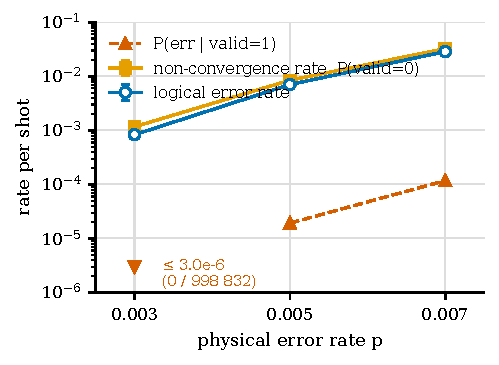
\includegraphics[width=\linewidth]{herald}
\caption{Logical error rate and non-convergence rate
$r(p)=P(\texttt{valid\_flag}=0)$ per physical error rate $p$, block path,
$10^{6}$ shots per point. The two curves nearly coincide because almost every
logical error is a non-converged shot: the attributable fraction $A(p)$ is
1.0000 / 0.9973 / 0.9960 at $p = 0.003$ / 0.005 / 0.007, and the error rate
conditioned on convergence is $\leq 3.0\times10^{-6}$ (zero observed in
998\,832 converged shots), $1.9\times10^{-5}$ and $1.2\times10^{-4}$.}
% src: docs/qec/q7-07-nonconvergence-policy.md "The ceiling — A(p), and what it forbids"
\label{fig:herald}
\end{figure}

% src: docs/superpowers/specs/2026-07-25-q7-07-nonconvergence-policy-design.md "Pre-registered decision rule"
% src: docs/qec/q7-07-nonconvergence-policy.md "The verdict, and the gap in the pre-registered rule"
Because $A \approx 1$, an oracle fallback acting only on flagged shots could
in principle remove the whole LER, so a fallback cannot be dismissed by
arithmetic; the decision rule, fixed before the data were seen, required a
candidate to show a significant paired rescue on the non-converged subset
and fit the latency budget.
% src: docs/qec/q7-07-nonconvergence-policy.md "AC-2 — candidate evaluation on the retained corpora"; "LER impact of every candidate, propagated"
We retained 1\,000 non-converged shots per point as a fixed corpus and
re-decoded each with five ordered-statistics-decoding (OSD) candidates:
OSD-0, OSD-2, OSD-4, and residual-restricted OSD-2 and OSD-4 (1, 4, 16, 4
and 16 solves per shot). Every candidate is worse than the baseline at every
point, and significantly so under a paired McNemar test (every $\chi^2 >
3.84$; the best row, residual OSD-4 at $p = 0.003$, rescues 116 shots and
breaks 169, $\chi^2 = 9.49$). Propagated as $\Delta\mathrm{LER} =
r(p)\,[P(\mathrm{err}\mid v{=}0) - P(\mathrm{err}\mid v{=}0,\mathrm{fallback})]$,
the candidates raise LER by between $+5.4\,\%$ and $+39.9\,\%$; OSD-0 turns
a 71\,\% conditional error rate into 99.6\,\%. The reason is that the BP
posteriors that order OSD's reliable basis are exactly the ones that just
failed to converge: forcing $H\hat{e} = s$ lands the solution in the wrong
logical class.
% src: docs/qec/q7-07-nonconvergence-policy.md "Latency, and a caveat about the parallel timing column"
The candidates also fail on latency: single-threaded on an EPYC 8124P, a
processor-side tail costs \SIrange{1460}{1644}{\micro\second} per shot it
fires on (including the software re-decode the flag-only RTL export forces),
against a \SI{1}{\micro\second}-per-round budget; a tail that fires on
0.12\,\% of shots still sets the worst case.
% src: docs/qec/q7-07-nonconvergence-policy.md "Chosen policy"
The chosen policy is therefore \emph{do-nothing-but-flag}: emit the best-kept
decision, export \texttt{valid\_flag}, no RTL change. Its LER impact is zero
by construction. This is reached for the opposite reason to the one the
rule's first branch anticipated (``non-convergence is negligible''):
non-convergence is nearly the entire error budget, and nothing affordable
recovers any of it. The two directions that could---more relay legs on a
flagged shot, or escalation to a host for non-real-time use---are outside
this work.

% src: docs/qec/q7-07-nonconvergence-policy.md "Board confirmation — the flag itself is bit-exact on silicon"
Finally, the flag the policy rests on is the silicon's flag. On the
matched-prior $p = 0.005$ overlay, $10^{5}$ fresh shots gave identical LER
in software and hardware ($7.1200\times10^{-3}$, 712 errors each), 0/100\,000
observable divergences, and 857 non-converged shots (0.857\,\%) on both
sides with \texttt{valid\_mismatch} $= 0$. This is one overlay, one operating
point and the block path only; at the other two points the licence remains
the observable-level bit-exactness of Table~\ref{tab:campaign} plus the
off-board co-simulation gate, which compares the flag.

\subsection*{Power}

% src: docs/perf/qec-q7-fixed-bp.md "Q7-05 — KV260 power / energy per decode (INA260, SOM-total)" / "Method"
The Kria K26 SOM exposes a single INA260 monitor on its \SI{5}{\volt} input
rail, so the only observable is SOM-total power (PS, PL, DDR and fan); there
is no PL-domain shunt. The measurement is therefore a delta between the PL
programmed-but-idle and the PL under a sustained decode stream, with a
processor-poll-only control (MMIO reads, no decode) to bound the share of the
delta owed to the host loop.
% src: docs/perf/qec-q7-fixed-bp.md "Q7-05" / "Results (two runs ...)"
On the shipped 16/48 overlay at \SI{133.332}{\MHz}, idle SOM power is
\SI{3.25}{\watt} (\SI{5.07}{\volt} $\times$ \SI{0.64}{\ampere}); a
full-schedule decode stream through the AXI4-Lite runner lifts it to
\SI{3.50}{\watt} ($+\SI{249}{\milli\watt}$, 2\,887 decodes/s, PL duty
4.5\,\%), early exit to \SI{3.46}{\watt} ($+\SI{210}{\milli\watt}$, duty
0.4\,\%), and the poll-only control alone to \SI{3.45}{\watt}
($+\SI{200}{\milli\watt}$). Two runs reproduce to $\pm\SI{5}{\milli\watt}$.
The host loop is thus about 80\,\% of the load delta; the decode datapath
adds only $\sim$\SI{48}{\milli\watt} (full) and $\sim$\SI{10}{\milli\watt}
(early exit) at the SOM level.
% src: docs/perf/qec-q7-fixed-bp.md "Q7-05" / "Energy per decode — two honest framings"
Energy per decode follows in two framings. As shipped through the per-word
harness, $\Delta P \cdot$ wall-per-decode is $\approx\SI{86}{\micro\joule}$
(full schedule) and $\approx\SI{67}{\micro\joule}$ (early exit); this is real
but harness-bound. Subtracting the control gives a PL-core dynamic energy of
$\lesssim\SI{17}{\micro\joule}$ (full) and $\lesssim\SI{3}{\micro\joule}$
(early exit), equivalent to about \SI{1}{\watt} of active PL power over the
\SI{15.64}{\micro\second} busy window. These are order-of-magnitude upper
bounds: they are a small difference of two $\sim$\SI{200}{\milli\watt}
numbers, and the control's read mix does not exactly match the decode
loop's. The batched DMA path raises the PL duty well above 4.5\,\% and would
turn the bound into a tight number; that re-measurement has not been done.

% 05-scaling — Scaling to the full-parallel geometry and a predictive ASIC.
% Every number carries a `% src:` comment naming the docs/ report and heading it was read from.
% Nothing here is a new measurement; nothing predictive is called "the chip".

\section{Scaling to the full-parallel geometry and a predictive ASIC}
\label{sec:scaling}

The shipped 16/48 core (\S\ref{sec:silicon}) decodes a worst-case window in 2085
cycles, \SI{15.64}{\micro\second} at the KV260's \SI{133.3}{\mega\hertz}.
% src: docs/perf/q7-02-ngroup-sweep.md "What this measures and why"
Latency is cycles divided by clock, so the two questions this section answers
are how far the cycle count can be pushed down by widening the core, and how
far the clock can be pushed up by leaving the FPGA. Both were measured rather
than modelled, and two of the three answers came out worse than the plan
assumed. We report them in the order they were obtained.

\subsection*{The banking family is the only implementable one}

Two architectures span the design space between the banked core and a fully
unrolled one. \texttt{bp\_relay\_unroll\_pipe} stamps $1/\mathit{NGROUP}$ of
the check and variable slots and time-multiplexes each across $\mathit{NGROUP}$
groups per BP phase. Its cycle count is exactly affine,
$\mathrm{cycles}(\mathit{NGROUP}) = 122\cdot\mathit{NGROUP}+240$, and the
co-simulation is 40/40 bit-identical to the golden at every setting measured.
% src: docs/perf/q7-02-ngroup-sweep.md "The cycle half: closed form, bit-exact everywhere"
The knob nevertheless has no feasible setting. Five values were synthesised
out-of-context on the KV260 part at a \SI{5.0}{\nano\second} target: every one
is over the device budget \emph{and} slower than the banked core. The cheapest
member, $\mathit{NGROUP}=144$ with one check slot and six variable slots
stamped, still needs 703\,698 LUTs (601\,\% of the device) at
\SI{17.5}{\mega\hertz}; the fastest, $\mathit{NGROUP}=16$, reaches
\SI{132.8}{\micro\second} at 1474\,\% of the device, 8.5$\times$ slower than
the shipped core. F$_{\max}$ is flat at 16.5--\SI{17.5}{\mega\hertz} across a
9$\times$ span of the knob.
% src: docs/perf/q7-02-ngroup-sweep.md "The area/Fmax half: measured"
The reason is structural: each slot gathers across $\mathit{NGROUP}$ groups and
there are $\texttt{BP\_C}/\mathit{NGROUP}$ slots, so the mux volume is
$\mathit{NGROUP}$-invariant by construction and the crossbar is simultaneously
the area floor and the critical path. Least squares gives
$\mathrm{LUT} = 615\,985 + 18\,415\,474/\mathit{NGROUP}$ within 5.7\,\%.
% src: docs/perf/q7-02-ngroup-sweep.md "Why: the crossbar is NGROUP-invariant by construction"
Banking, which replaces the flat register array plus crossbar with
index-addressed banks, is therefore not an optimisation of a working parallel
design but the thing that makes it implementable.
% src: docs/perf/q7-02-ngroup-sweep.md "Consequences"

Within the banked family the plan had assumed cycles scale linearly with bank
count. Cycle-measuring five geometries showed that they do not. The counts fit
the exact closed form
\begin{equation}
  \mathrm{cycles} = 60\,(G_C+G_V) + 420 + (2G_V + G_C),
  \label{eq:cycles}
\end{equation}
where $G_C,G_V$ are the check and variable group counts and the constant
$420 = 60\cdot 7$ is a per-iteration pipeline tail (seven drain cycles in each
of the $\mathrm{LEGS}\cdot\mathrm{ITERS}=60$ iterations) that exists regardless
of banking. Only the first term shrinks with banking, so 4$\times$ banking
(16/48 $\to$ 64/192) yields 2.28$\times$ fewer cycles, 2085 $\to$ 913, and the
tail grows from 20\,\% to 47\,\% of the budget.
% src: docs/qec/asic-architecture.md "Banking-scaling qualification (measured, Q7-08 follow-up)"
The floor is the full-parallel geometry, $G_C=G_V=1$: 543 cycles. This
configuration could not be generated when the qualification was written; three
generator defects (routing-network lanes sized by bank count rather than tap
count, a zero-width row address at $\lceil\log_2 1\rceil=0$, and ROM literals
beyond Verilator's 65\,536-bit limit) were fixed in Task~B0 Option~A, after
which 48/288, 144/432 and 144/864 all pass the 40-shot golden 40/40 at 789, 605
and 543 cycles, with the header for every previously qualified geometry
byte-identical apart from two guard lines.
% src: docs/qec/open-silicon-program.md "Task B0 Option A RESULT (2026-07-30)"
Since the 420-cycle tail is $\mathrm{LEGS}\cdot\mathrm{ITERS}\cdot 7$, the
dominant remaining latency lever once banking is exhausted is the iteration
budget, ITERS, which is set by the decoder's LER at the operating point rather
than by the hardware.
% src: docs/qec/asic-architecture.md "Banking-scaling qualification (measured, Q7-08 follow-up)"

\subsection*{A large FPGA: it fits, and the clock collapses}

Both 64/192 and 144/864 were implemented end to end (synthesis, opt, place,
phys\_opt, route) on the AMD Virtex UltraScale+ HBM \texttt{xcvu47p-fsvh2892-2-e}
of AWS's F2 instances, with Vivado 2025.2 on a \texttt{z1d.2xlarge} build
instance, at a \SI{5.0}{\nano\second} target, default directives, no
floorplanning and no fanout constraints. The instance lived 7.3 hours and cost
about \$5.50; 64/192 implemented in 65 minutes, 144/864 in 5\,h\,40\,min.
% src: docs/perf/q7-02-fullparallel-fpga.md "8. What was run"
No FPGA instance was rented: the build only needs the Vivado Enterprise licence
that the FPGA Developer AMI bundles, and a bitstream is never loaded.
% src: docs/qec/b2-aws-build-runbook.md "What you are renting and why"
Table~\ref{tab:fpga} gives the post-route result.

\begin{table}[t]
  \centering
  \footnotesize
  \caption{Post-route implementation of two banked geometries on the VU47P
    (Vivado 2025.2, \SI{5.0}{\nano\second} target, default directives). The
    shipped KV260 row is the silicon measurement of \S\ref{sec:silicon}.}
  \label{tab:fpga}
  \begin{tabular}{@{}lrrrrr@{}}
    \toprule
    Geometry & Cycles & LUTs & Util. & F$_{\max}$ & Latency \\
             &        &      & (\%)  & (MHz)      & (\si{\micro\second}) \\
    \midrule
    64/192   & 913  & 247\,434 & 19.0 & 150.4 & 6.07 \\
    144/864  & 543  & 994\,700 & 76.3 & 97.3  & 5.58 \\
    \addlinespace
    16/48, KV260 & 2085 & --- & --- & 133.3 & 15.64 \\
    \bottomrule
  \end{tabular}
  % src: docs/perf/q7-02-fullparallel-fpga.md "9. Results"
\end{table}

The fit gate passes: 76.3\,\% is under the 90\,\% criterion, BRAM and LUTRAM
are at zero and registers at 9.4\,\%, so LUTs are the only resource that
matters. The latency case for full-parallel on FPGA does not pass:
1.68$\times$ fewer cycles at a 1.55$\times$ slower clock is a net 1.09$\times$
for 4.0$\times$ the area. 64/192 delivers 92\,\% of the latency in a quarter of
the device.
% src: docs/perf/q7-02-fullparallel-fpga.md "9. Results"
The clock loss is not logic depth. The worst path has eight logic levels and a
\SI{10.251}{\nano\second} data-path delay of which \SI{0.750}{\nano\second}
(7.3\,\%) is logic and \SI{9.501}{\nano\second} (92.7\,\%) is routing: a
control counter, \texttt{pc\_reg[1]}, reaching a min-sum cell across a die large
enough to need three super logic regions, with Laguna SLR-crossing tiles inside
the congested windows. It is the fanout-7941 control net the out-of-context
probe had flagged, and every standard mitigation (\texttt{MAX\_FANOUT}, per-bank
replication, SLR-aware floorplanning) is untried, so \SI{97.3}{\mega\hertz} is
a floor for this design rather than its ceiling.
% src: docs/perf/q7-02-fullparallel-fpga.md "10. Why the clock collapsed"
Two calibration lessons are worth carrying forward. The same RTL synthesised to
803\,518 CLB LUTs on the KV260 part with Vivado 2024.2 and to 1\,000\,035 on the
VU47P with 2025.2, 24\,\% more, so cross-part LUT extrapolation is worth about
$\pm25\,\%$; and post-route utilisation moved less than 1\,\% off
post-synthesis on this part.
% src: docs/perf/q7-02-fullparallel-fpga.md "11. Where Step 0's projections were wrong"
% src: docs/perf/q7-02-fullparallel-fpga.md "9. Results"
Sub-microsecond needs \SI{543}{\mega\hertz} on 543 cycles; nothing in this
family on any FPGA is within a factor of three of that.
% src: docs/perf/q7-02-fullparallel-fpga.md "4. Calibration"

\subsection*{7\,nm predictive: the geometry penalty is mostly an FPGA artefact}

The FPGA result raised a specific risk: the only ASIC-node clock this project
had measured, \SI{686.13}{\mega\hertz}, came from the 16/48 geometry, and the
program had been quoting 543 cycles against it as if the clock were
geometry-independent.
% src: docs/perf/q7-02-fullparallel-fpga.md "12. What this means for the ASIC"
Both geometries were therefore run through OpenROAD-flow-scripts
\citep{openroad} on the ASAP7 predictive 7\,nm platform \citep{clark2016asap7},
with the Q7-08 latch register file, identical knobs
(\texttt{CORE\_UTILIZATION}=45, \texttt{PLACE\_DENSITY}=0.55, SDC period
\SI{1000}{\pico\second}, timing repair skipped because \texttt{repair\_timing}
segfaults on this netlist class), and RC-extracted post-route timing. The
144/864 run took about 20 hours on an EPYC box and completed with $rc=0$.
% src: docs/perf/q7-02-b3-asap7-fullparallel.md "1. What was run"
Table~\ref{tab:asap7} summarises both.

\begin{table}[t]
  \centering
  \small
  \caption{ASAP7 7\,nm predictive, post-route, same flow and knobs for both
    geometries. F$_{\max}$ is \texttt{report\_clock\_min\_period}, setup-only,
    on a netlist whose hold violations are unrepaired (\S\ref{sec:limitations}).
    Power is from a gate-level VCD of the 16/48 netlist at the
    \SI{1}{\giga\hertz} SDC; it was not measured at 144/864.}
  \label{tab:asap7}
  \begin{tabular}{@{}lrr@{}}
    \toprule
    & 16/48 & 144/864 \\
    \midrule
    Cycles (worst case)                & 2085   & 543 \\
    Design area at 50\,\% util. (\si{\micro\metre\squared}) & 81\,090 & 434\,450 \\
    Die (\si{\milli\metre\squared})    & 0.163  & 0.869 \\
    F$_{\max}$, setup-only (MHz)       & 686.13 & 614.59 \\
    WNS at \SI{1000}{\pico\second} (ps) & $-622.73$ & $-1117.97$ \\
    Latency (\si{\micro\second})       & 3.04   & 0.88 \\
    DRC violations                     & 0      & 0 \\
    Hold violations (unrepaired)       & 44\,704 & 35\,616 \\
    \addlinespace
    Power, steady BP (W)               & 0.149  & --- \\
    Power, idle, clock running (W)     & 0.138  & --- \\
    Energy per 2085-cycle window (\si{\micro\joule}) & 0.31 & --- \\
    \bottomrule
  \end{tabular}
  % src: docs/perf/q7-02-b3-asap7-fullparallel.md "2. Results, against the 16/48 baseline"
  % src: docs/perf/q7-02-asap7-timing.md "7. Closure note" (0.163 mm^2 die)
  % src: docs/perf/q7-02-b3-asap7-fullparallel.md "3.2 Neither run had timing repair" (hold counts)
  % src: docs/perf/q7-02-asap7-timing.md "4. Power" (power rows)
\end{table}

The clock is geometry-dependent on the ASIC too, but only mildly: the step from
the small to the full-parallel geometry costs $-10.4\,\%$ on ASAP7 against
$-35.3\,\%$ on the VU47P. An ASIC has neither fixed routing tracks nor SLR
boundaries, and its buffer trees absorb the high-fanout control net that
dominated the FPGA path; roughly a third of the penalty transferred. Area scales
sub-linearly, 5.36$\times$ for 8.5$\times$ the logic, where the FPGA paid
8.53$\times$ in CLB LUTs; of the placer's $+11.18\,\%$ over the raw netlist,
routability inflation was $+1.28\,\%$ and timing-driven growth $+9.90\,\%$.
% src: docs/perf/q7-02-b3-asap7-fullparallel.md "2. Results" ("The geometry penalty", "Area scales sub-linearly")
The headline, $543\ \text{cycles} / \SI{614.59}{\mega\hertz} =
\SI{0.88}{\micro\second}$, is a sub-microsecond worst-case window on a 7\,nm
predictive node, DRC-clean, at \SI{0.869}{\milli\metre\squared}.
% src: docs/perf/q7-02-b3-asap7-fullparallel.md "4. Verdict"
Figure~\ref{fig:latency} places it against the FPGA points.

We state the two qualifications here rather than only in
\S\ref{sec:limitations}. First, every F$_{\max}$ in Table~\ref{tab:asap7} is a
\emph{setup-only} figure: hold was never repaired, the 16/48 netlist carries
44\,704 hold violations (worst \SI{-745.9}{\pico\second}, 98\,\% on the D pins
of the latch register file) and the 144/864 netlist 35\,616 (worst
\SI{-1486.9}{\pico\second}). Hold does not scale with the clock period, so
these netlists would not decode correctly at any frequency; the first
gate-level co-simulation of the 16/48 netlist fails 40/40 in exactly the way
STA predicts, and \SI{686}{\mega\hertz} is the speed of the datapath, not of a
working part. A separately repaired but unrouted run gave
\SI{527.66}{\mega\hertz}, so the defensible 16/48 band is
528--\SI{686}{\mega\hertz}.
% src: docs/perf/q7-02-asap7-timing.md "1. Headline: the Fmax number straddles the budget"
% src: docs/perf/q7-02-asap7-timing.md "4b. Gate-level co-simulation"
Second, ASAP7 is a proxy: the margin below \SI{1}{\micro\second} is 12\,\%, a
1.2$\times$ node penalty gives \SI{1.06}{\micro\second}, and nothing in this
work measures the gap to a production node.
% src: docs/qec/open-silicon-program.md "4. Risk register" ("The node")

\subsection*{Power with real switching activity}

The default-activity power ORFS reports, \SI{0.656}{\watt}, is not a decoder
number. The routed 16/48 netlist (639\,322 cells, among them 55\,703 latches
and 43\,025 flops) was compiled with Verilator against the ASAP7 behavioural
cell models and driven by the same testbench and 40 golden vectors the RTL
passes; two 300-cycle VCD windows, one inside a steady-state BP iteration and
one with the decoder parked, were fed to OpenSTA with the extracted SPEF,
annotating 2\,128\,987 pin activities with none left unannotated.
% src: docs/perf/q7-02-asap7-timing.md "4. Power — measured with real switching activity (Task A4)"
At the \SI{1}{\giga\hertz} SDC the core draws \SI{0.149}{\watt} during BP and
\SI{0.138}{\watt} idle; the default activity was 4.4$\times$ too high, almost
entirely in the combinational group (\SI{0.466}{\watt} $\to$
\SI{0.0115}{\watt}). Ninety-three per cent of the real power is clock tree
plus sequential internal: the ASAP7 platform marks integrated clock-gating
cells \texttt{DONT\_USE}, so every register toggles its clock pin every cycle
and the datapath itself is about \SI{10}{\milli\watt}. Energy per worst-case
window is \SI{149}{\pico\joule} per cycle $\times$ 2085 cycles $=$
\SI{0.31}{\micro\joule}, clock-independent to first order and inside the
\SI{1}{\micro\joule} budget with 3$\times$ margin, at 7\,nm predictive; the
activity comes from the not-quite-bit-exact simulation of the previous
paragraph, and absolute watts on a predictive NLDM library should be read as
$\pm30\,\%$.
% src: docs/perf/q7-02-asap7-timing.md "4. Power — measured with real switching activity (Task A4)"

\begin{figure}[t]
  \centering
  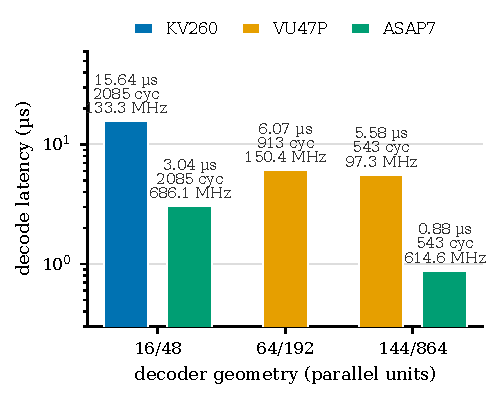
\includegraphics[width=\linewidth]{latency.pdf}
  \caption{Worst-case decode latency against banking geometry on the three
    platforms measured: KV260 silicon (16/48), VU47P post-route (64/192,
    144/864) and ASAP7 7\,nm predictive post-route (16/48, 144/864). ASAP7
    points are setup-only clocks on hold-unrepaired netlists. Data as in
    Tables~\ref{tab:fpga} and~\ref{tab:asap7}.}
  \label{fig:latency}
\end{figure}

\section{Limitations and negative results}
\label{sec:limitations}

We list these with the same weight as the positive results; several redirected the design.

\paragraph{Hold on the latch register file.}
% src: docs/perf/q7-02-asap7-timing.md §4b, §7
The routed 16/48 ASAP7 netlist has 44\,704 hold violations (worst \SI{-745.9}{\pico\second}), 43\,802
of them on the D pins of the latch register file: the latch write pulse is derived from
\texttt{we \& \textasciitilde{}clk} and realised as a clock-tree sub-network with \SI{1.37}{\nano\second}
insertion delay against \SI{0.47}{\nano\second} for the flip-flops, so the latches close about
\SI{0.9}{\nano\second} after the flops launch new data. The first gate-level co-simulation of the
netlist reproduces the consequence: the 2085-cycle schedule runs exactly on all 40 golden shots, but
8--15 of 877 output fields differ and the decode does not converge. Hold is independent of clock
period, and \texttt{repair\_timing -hold} would need on the order of $10^6$ delay buffers
(\texttt{DPL-0038}); the fix is an integrated clock-gating cell or a re-timed write pulse, which the
ASAP7 platform's \texttt{DONT\_USE ICG*} setting precluded here. Until it is made, every frequency
in \S\ref{sec:scaling} is a setup-only datapath figure, and the same un-gated clock is why
\SI{93}{\percent} of the measured power is register clocking. The 144/864 netlist carries the same
defect (35\,616 violations, worst \SI{-1486.9}{\pico\second}).

\paragraph{7\,nm predictive is not a target node.}
% src: docs/qec/open-silicon-program.md risk register; docs/perf/q7-02-b3-asap7-fullparallel.md §3.1
ASAP7 \citep{clark2016asap7} is a research kit. The margin between \SI{0.88}{\micro\second} and the
microsecond is \SI{12}{\percent}; a $1.2\times$ node penalty at 28\,nm would erase it. Nothing in this
work measures that gap, and a 28\,nm PDK is a gate we have not passed.

\paragraph{The streaming core does not fit.}
% src: docs/qec/open-silicon-program.md §1.2; memory of M9c verdict in docs/perf/qec-q7-fixed-bp.md
A windowed streaming variant with a runtime-addressed gather reached \SI{162}{\percent} of the KV260's
LUTs and \SI{113}{\percent} of its BRAM by estimate and exhausted \SI{123}{\giga\byte} of host memory
in technology mapping. It is bit-exact in simulation only; the fixed-permutation gather of
\S\ref{sec:architecture} is the answer to it, not a refinement of it.

\paragraph{No OSD tail; no \texttt{NGROUP}.}
% src: docs/perf/qec-q7-fixed-bp.md "OSD-0 tail"; docs/perf/q7-02-ngroup-sweep.md
An OSD-0 post-processor did not reduce the logical error rate at the operating points measured, and
the order-12 sweep that would has no place in a microsecond budget. A grouped partial-unroll knob
(\texttt{NGROUP}) has no setting that both fits and is faster than the banked core.

\paragraph{Uncovered corners.}
% src: docs/perf/q7-02-asap7-timing.md §7
Runt frames (fewer slices than the window) take a zero-pad path that no co-simulation vector
exercises; the 64/192 and 144/864 geometries have been cycle-counted and synthesised but not run on
hardware we own; and the gate-level co-simulation used behavioural replacements for two sequential
cells because the vendor UDP models cannot be compiled by Verilator (an event-driven arbitration with
the vendor models was attempted and remained X-contaminated).

\paragraph{One author, one lab.}
All measurements were made by the author on the author's hardware. The deployment procedure has been
executed on three wiped boards, but not yet by a third party; the repository invites and documents
exactly that.

% 07-reproducibility — to be written


\bibliographystyle{unsrtnat}
\bibliography{refs}

\appendix
\onecolumn
\section{Provenance of every number}
\label{app:prov}

Each numeric claim in the text carries, in the \LaTeX{} source, a comment naming the repository
file and heading it was copied from. This table lists those files per section (headings
abbreviated); the reports themselves are in \texttt{docs/} of the repository \citep{alephrepo}
at the commit tagged \texttt{preprint-v1}; the section headings quoted in each comment locate the
exact table or paragraph.

\begin{footnotesize}
\begin{tabular}{@{}p{0.16\textwidth}>{\raggedright\arraybackslash}p{0.80\textwidth}@{}}
\toprule
Section & Source files (\texttt{docs/} unless noted) \\
\midrule
\S2 The decoder & \texttt{perf/qec-q5-gross.md}; \texttt{perf/qec-q5-circuit-dem.md}; \texttt{perf/qec-q7-fixed-bp.md}; \texttt{perf/qec-q5-bposd.md}; \texttt{perf/data/qec-q7-fixed-bp.csv}; \texttt{perf/data/qec-q7-budget.csv} \\[2pt]
\S3 Hardware architecture & \texttt{perf/qec-q7-fixed-bp.md}; \texttt{superpowers/specs/2026-07-15-m9c-serial-gather-design.md}; \texttt{superpowers/specs/2026-07-16-m9c-aswaksman-rightsize-design.md}; \texttt{qec/asic-architecture.md}; \texttt{qec/regfile-plan.md}; \texttt{qec/q7-06-ac1-batched-dma.md}; \texttt{perf/q7-02-asap7-timing.md} \\[2pt]
\S4 Results on FPGA silicon & \texttt{perf/qec-q7-fixed-bp.md}; \texttt{hw/product/README.md}; \texttt{hw/product/interface-spec.md}; \texttt{qec/q7-06-ac1-batched-dma.md}; \texttt{qec/q7-07-nonconvergence-policy.md}; \texttt{superpowers/specs/2026-07-25-q7-07-nonconvergence-policy-design.md} \\[2pt]
\S5 Scaling and predictive ASIC & \texttt{perf/q7-02-ngroup-sweep.md}; \texttt{qec/asic-architecture.md}; \texttt{qec/open-silicon-program.md}; \texttt{perf/q7-02-fullparallel-fpga.md}; \texttt{qec/b2-aws-build-runbook.md}; \texttt{perf/q7-02-b3-asap7-fullparallel.md}; \texttt{perf/q7-02-asap7-timing.md} \\[2pt]
\S6 Limitations & \texttt{perf/q7-02-asap7-timing.md}; \texttt{qec/open-silicon-program.md}; \texttt{perf/q7-02-b3-asap7-fullparallel.md}; \texttt{perf/qec-q7-fixed-bp.md}; \texttt{perf/q7-02-ngroup-sweep.md} \\[2pt]
\S7 Reproducibility & \texttt{hw/product/README.md} \\[2pt]
\bottomrule
\end{tabular}
\end{footnotesize}

\end{document}
